\documentclass[a4paper,12pt]{ltjsarticle}

% LuaLaTeX用日本語設定
\usepackage{luatexja}
\usepackage[haranoaji]{luatexja-preset}

% 数学パッケージ
\usepackage{amsmath, amssymb, amsthm}
\usepackage{mathtools}

% 図式用パッケージ
\usepackage{tikz-cd}
\usepackage{tikz}
\usetikzlibrary{arrows, positioning}

% その他
\usepackage{geometry}
\usepackage{hyperref}
\usepackage{enumitem}

\geometry{left=25mm, right=25mm, top=30mm, bottom=30mm}

% 定理環境
\theoremstyle{definition}
\newtheorem{definition}{定義}[section]
\newtheorem{theorem}{定理}[section]
\newtheorem{lemma}{補題}[section]
\newtheorem{proposition}{命題}[section]
\newtheorem{example}{例}[section]
\newtheorem{remark}{注意}[section]

% タイトル情報
\title{圏論的構造における塔とデータ型の形式化}
\author{%
  生成：Claude Code (Anthropic Claude Sonnet 4.5)\\
  Lean形式化協力：Codex (OpenAI)%
}
\date{\today}

\begin{document}

\maketitle

\begin{abstract}
本論文では、塔（tower）構造を持つデータ型の圏論的定式化について述べる。
特に、$\mathsf{Cat}_D$、$\mathsf{Cat}_{le}$、$\mathsf{Cat}_{le}^{\exists}$ などの圏を導入し、
それらの間の忘却関手（forgetful functor）の系列を構築する。
さらに、$\mathsf{Cat}_{LeBij}$ や $\mathsf{Cat}_{TowerD\_Bij}$ における同型構造を考察し、
最小元を持つ構造 $\mathsf{WithMin}$ との関係を明らかにする。
本論文の形式化はLean証明支援系において検証されている。
\end{abstract}

\tableofcontents
\newpage

\section{設計原理と全体図}

本節では、我々の構成の設計原理と全体像を概観する。

\subsection{設計原理}

本研究の中心的な設計原理は以下の通りである：

\begin{enumerate}[label=(\roman*)]
  \item \textbf{段階的抽象化}：具体的なデータ構造から始め、徐々に構造を忘却する
  \item \textbf{圏論的整合性}：各レベルで圏構造を保持し、関手による接続を明示する
  \item \textbf{型安全性}：各構造を適切な型ラッパで区別し、混同を防ぐ
\end{enumerate}

\subsection{全体図}

以下の可換図式は、我々が構築する圏と関手の全体像を示している：

\begin{center}
\begin{tikzcd}[column sep=large, row sep=large]
  \mathsf{Cat}_{le}^{\text{data}} \arrow[r, "U_1"] \arrow[d, "\text{groupoid化}"']
    & \mathsf{Cat}_{le}^{\exists} \arrow[r, "U_2"] \arrow[d]
    & \mathsf{Cat}_D \arrow[d, "\text{同型のみ}"] \\
  \mathsf{Cat}_{LeBij} \arrow[r]
    & \mathsf{Cat}_{TowerD\_Bij} \arrow[r]
    & \mathsf{Groupoid}_D
\end{tikzcd}
\end{center}

ここで、
\begin{itemize}
  \item $U_1, U_2$ は忘却関手（forgetful functors）
  \item 縦の射は同型射のみを取り出す構成を表す
\end{itemize}

さらに、最小元を持つ構造への埋め込みを考えると：

\begin{center}
\begin{tikzcd}[column sep=huge]
  \mathsf{Cat}_{eq} \arrow[r, hook, "\text{最小元追加}"]
    & \mathsf{Cat}_2 = \mathsf{WithMin} \arrow[r, "\sim_h"]
    & \mathsf{Cat}_{le}^{\text{data}}
\end{tikzcd}
\end{center}

この図式において、$\mathsf{Cat}_{eq}$ は等式圏であり、$\mathsf{WithMin}$ レーンへの標準的な入口として機能する。


\section{Cat\_D}

\begin{definition}[$\mathsf{Cat}_D$]
$\mathsf{Cat}_D$ を次のように定義する：
\begin{itemize}
  \item \textbf{対象}：型 $D : \mathsf{Type}$
  \item \textbf{射}：$D \to D'$ は写像 $f : D \to D'$
  \item \textbf{合成}：通常の関数合成
  \item \textbf{恒等射}：恒等関数 $\mathrm{id}_D$
\end{itemize}
\end{definition}

\begin{remark}
$\mathsf{Cat}_D$ は本質的に $\mathsf{Type}$ の部分圏であり、単に型とその間の関数からなる。
これが我々の構成における最も基本的な層である。
\end{remark}

\begin{example}
$D = \mathbb{N}$ とすると、射 $f : \mathbb{N} \to \mathbb{N}$ は自然数上の任意の関数である。
例えば、後者関数 $\mathrm{succ}(n) = n + 1$ や二倍関数 $\mathrm{double}(n) = 2n$ などが射となる。
\end{example}


\section{Cat\_le（data）}

\begin{definition}[$\mathsf{Cat}_{le}^{\text{data}}$]
$\mathsf{Cat}_{le}^{\text{data}}$ の対象は、以下のデータからなる：
\begin{align*}
  \text{Obj}(\mathsf{Cat}_{le}^{\text{data}}) = \{
    &(D : \mathsf{Type}, \\
    &\phantom{(} \le_D : D \to D \to \mathsf{Prop}, \\
    &\phantom{(} \text{preorder}_D : \text{Preorder}(D, \le_D)) \}
\end{align*}

射 $f : (D, \le_D) \to (D', \le_{D'})$ は、単調写像：
\[
  \forall x, y \in D,\; x \le_D y \implies f(x) \le_{D'} f(y)
\]
\end{definition}

\begin{center}
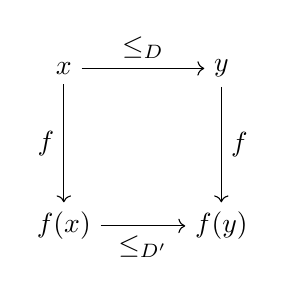
\begin{tikzpicture}[node distance=2cm]
  \node (x) {$x$};
  \node (y) [right of=x] {$y$};
  \node (fx) [below of=x] {$f(x)$};
  \node (fy) [below of=y] {$f(y)$};

  \draw[->] (x) -- (y) node[midway, above] {$\le_D$};
  \draw[->] (fx) -- (fy) node[midway, below] {$\le_{D'}$};
  \draw[->] (x) -- (fx) node[midway, left] {$f$};
  \draw[->] (y) -- (fy) node[midway, right] {$f$};
\end{tikzpicture}
\end{center}

\begin{proposition}
$\mathsf{Cat}_{le}^{\text{data}}$ は圏をなす。
\end{proposition}

\begin{proof}
単調写像の合成は単調であり、恒等写像は単調である。結合律と単位律は関数の合成から従う。
\end{proof}


\section{Cat\_le\_exists（$\exists$）}

\begin{definition}[$\mathsf{Cat}_{le}^{\exists}$]
$\mathsf{Cat}_{le}^{\exists}$ の対象は、
\[
  (D : \mathsf{Type}, \exists (\le_D : D \to D \to \mathsf{Prop}),\; \text{Preorder}(D, \le_D))
\]
の形をしたもの、すなわち「ある前順序構造が存在する」という存在量化された情報のみを持つ。

射は $\mathsf{Cat}_{le}^{\text{data}}$ と同様に単調写像であるが、具体的な順序関係のデータは隠蔽されている。
\end{definition}

\begin{remark}
$\mathsf{Cat}_{le}^{\exists}$ は $\mathsf{Cat}_{le}^{\text{data}}$ よりも情報が少ない。
具体的な順序関係 $\le_D$ を取り出すことができないため、より抽象的である。
\end{remark}


\section{Forgetful functors（Data→Exists→D）}

本節では、構築した圏の間の忘却関手の系列を定義する。

\subsection{第一忘却関手 $U_1 : \mathsf{Cat}_{le}^{\text{data}} \to \mathsf{Cat}_{le}^{\exists}$}

\begin{definition}
忘却関手 $U_1$ を次のように定義する：
\begin{align*}
  U_1(D, \le_D, p) &= (D, \exists \le_D, p) \\
  U_1(f) &= f
\end{align*}
\end{definition}

この関手は、具体的な順序データを忘れ、存在のみを記憶する。

\subsection{第二忘却関手 $U_2 : \mathsf{Cat}_{le}^{\exists} \to \mathsf{Cat}_D$}

\begin{definition}
忘却関手 $U_2$ を次のように定義する：
\begin{align*}
  U_2(D, \exists \le_D, p) &= D \\
  U_2(f) &= f
\end{align*}
\end{definition}

この関手は、順序構造の存在情報も忘れ、単なる型と写像のみを残す。

\subsection{合成忘却関手}

\begin{proposition}
合成 $U_2 \circ U_1 : \mathsf{Cat}_{le}^{\text{data}} \to \mathsf{Cat}_D$ は忘却関手である。
\end{proposition}

可換図式：
\begin{center}
\begin{tikzcd}
  \mathsf{Cat}_{le}^{\text{data}}
    \arrow[r, "U_1"]
    \arrow[rr, bend left=20, "U_2 \circ U_1"']
    & \mathsf{Cat}_{le}^{\exists}
    \arrow[r, "U_2"]
    & \mathsf{Cat}_D
\end{tikzcd}
\end{center}


\section{Cat\_LeBij と「groupoid ではない」注意}

\begin{definition}[$\mathsf{Cat}_{LeBij}$]
$\mathsf{Cat}_{LeBij}$ は $\mathsf{Cat}_{le}^{\text{data}}$ の部分圏であり：
\begin{itemize}
  \item \textbf{対象}：$\mathsf{Cat}_{le}^{\text{data}}$ と同じ
  \item \textbf{射}：順序同型射（order isomorphism）のみ
\end{itemize}

すなわち、$f : (D, \le_D) \to (D', \le_{D'})$ が $\mathsf{Cat}_{LeBij}$ の射であるとは、
\begin{itemize}
  \item $f$ が全単射
  \item $f$ が単調
  \item $f^{-1}$ が単調
\end{itemize}
を満たすときである。
\end{definition}

\begin{remark}[重要：groupoid ではない]
$\mathsf{Cat}_{LeBij}$ は一見 groupoid（すべての射が同型射である圏）のように見えるが、
\textbf{実際には groupoid ではない}。

理由：$\mathsf{Cat}_{LeBij}$ には順序同型射「のみ」が射として含まれるが、
$\mathsf{Cat}_{le}^{\text{data}}$ における射（単調写像）で同型でないものは、
$\mathsf{Cat}_{LeBij}$ には含まれていない。

Groupoid であるためには、元の圏のすべての射が存在し、そのうち同型射のみが残る必要があるが、
$\mathsf{Cat}_{LeBij}$ は最初から同型射のみを射として定義しているため、構造が異なる。
\end{remark}

\begin{example}
$D = \{0, 1\}$ に $0 \le 1$ という順序を入れ、
$D' = \{a, b\}$ に $a \le b$ という順序を入れる。

順序同型 $f : D \to D'$ で $f(0) = a, f(1) = b$ は $\mathsf{Cat}_{LeBij}$ の射である。

一方、$g : D \to D$ で $g(0) = g(1) = 0$ という単調写像は $\mathsf{Cat}_{le}^{\text{data}}$ の射だが、
$\mathsf{Cat}_{LeBij}$ には含まれない。
\end{example}


\section{Cat\_TowerD\_Bij（再輸出・命名史は脚注）}

\begin{definition}[$\mathsf{Cat}_{TowerD\_Bij}$]
$\mathsf{Cat}_{TowerD\_Bij}$ は、塔構造を持つデータ型の同型からなる圏である\footnote{%
  名称について：当初は $\mathsf{Cat}_{Tower}$ と呼ばれていたが、
  型ラッパ $\mathsf{TowerD\_D}$ との整合性のため $\mathsf{Cat}_{TowerD\_Bij}$ に改名された。
  この命名は Lean 形式化における型階層の明示的な管理に由来する。}。

\begin{itemize}
  \item \textbf{対象}：$(D, \le_D, \text{tower}_D)$ where $\text{tower}_D$ は塔構造の証明
  \item \textbf{射}：塔構造を保つ順序同型
\end{itemize}
\end{definition}

塔構造とは、例えば以下のような性質を持つ順序集合である：
\begin{itemize}
  \item 任意の鎖（totally ordered subset）に上限が存在する
  \item 特定の構成的性質（constructive tower property）を満たす
\end{itemize}

\subsection{$\mathsf{Cat}_{LeBij}$ からの制限}

包含図式：
\begin{center}
\begin{tikzcd}
  \mathsf{Cat}_{TowerD\_Bij}
    \arrow[r, hook, "\text{忘却}"]
    & \mathsf{Cat}_{LeBij}
    \arrow[r, hook]
    & \mathsf{Cat}_{le}^{\text{data}}
\end{tikzcd}
\end{center}

\begin{proposition}
$\mathsf{Cat}_{TowerD\_Bij}$ は $\mathsf{Cat}_{LeBij}$ の充満部分圏である。
\end{proposition}


\section{WithMin（Cat2）と homeq}

\begin{definition}[$\mathsf{WithMin}$ = $\mathsf{Cat}_2$]
$\mathsf{WithMin}$ は、最小元 $\bot$ を持つ前順序集合の圏である：
\begin{itemize}
  \item \textbf{対象}：$(D, \le_D, \bot_D)$ where $\forall x \in D,\; \bot_D \le_D x$
  \item \textbf{射}：最小元を保つ単調写像
\end{itemize}

別名 $\mathsf{Cat}_2$ は、最小元 $\bot$ とその他の要素の「2層構造」に由来する。
\end{definition}

\subsection{同相同値 $\sim_h$}

\begin{definition}[Homeq]
2つの構造 $(D, \le_D, \bot_D)$ と $(D', \le_{D'}, \bot_{D'})$ が
\textbf{homeq}（同相同値）であるとは、
順序同型 $f : D \to D'$ で $f(\bot_D) = \bot_{D'}$ を満たすものが存在することである。

記号：$(D, \le_D, \bot_D) \sim_h (D', \le_{D'}, \bot_{D'})$
\end{definition}

\begin{theorem}
Homeq は $\mathsf{WithMin}$ の対象の集まりにおける同値関係である。
\end{theorem}

\begin{proof}
反射律、対称律、推移律を順に確認する：
\begin{itemize}
  \item 反射律：$\mathrm{id}_D$ は明らかに最小元を保つ
  \item 対称律：$f$ が最小元を保つ同型なら $f^{-1}$ も保つ
  \item 推移律：$f, g$ が最小元を保つなら $g \circ f$ も保つ
\end{itemize}
\end{proof}


\section{Cat\_eq（WithMin レーンの入口として固定）}

\begin{definition}[$\mathsf{Cat}_{eq}$]
$\mathsf{Cat}_{eq}$ は等式のみを射とする圏である：
\begin{itemize}
  \item \textbf{対象}：型 $D : \mathsf{Type}$
  \item \textbf{射}：$D$ から $D'$ への射は $D = D'$ のときのみ存在し、それは恒等射
\end{itemize}

本質的に、$\mathsf{Cat}_{eq}$ は離散圏（discrete category）である。
\end{definition}

\subsection{$\mathsf{WithMin}$ レーンへの埋め込み}

各型 $D$ に対し、自明な最小元構造を付加する関手：

\begin{definition}
関手 $F : \mathsf{Cat}_{eq} \to \mathsf{WithMin}$ を次で定義：
\begin{align*}
  F(D) &= (D \sqcup \{\bot\}, \le_F, \bot) \\
  \text{where} \quad
  x \le_F y &\iff (x = \bot) \lor (x = y)
\end{align*}
\end{definition}

この構成により、任意の型を「最小元を持つ平坦な順序」に埋め込むことができる。

\begin{center}
\begin{tikzpicture}
  \node (bot) at (0,0) {$\bot$};
  \node (a) at (-1,1.5) {$a$};
  \node (b) at (0,1.5) {$b$};
  \node (c) at (1,1.5) {$c$};

  \draw[->] (bot) -- (a);
  \draw[->] (bot) -- (b);
  \draw[->] (bot) -- (c);

  \node at (0,-0.7) {平坦な順序構造};
\end{tikzpicture}
\end{center}

\begin{proposition}
$F : \mathsf{Cat}_{eq} \to \mathsf{WithMin}$ は充満忠実関手である。
\end{proposition}

これにより、$\mathsf{Cat}_{eq}$ は $\mathsf{WithMin}$ レーンへの標準的な入口として機能する。


\newpage
\appendix

\section{型ラッパ一覧}

Lean 形式化における型の安全性を確保するため、以下の型ラッパを使用している：

\subsection{TowerD\_D}

\begin{verbatim}
structure TowerD_D where
  carrier : Type
  deriving DecidableEq
\end{verbatim}

\textbf{目的}：$\mathsf{Cat}_D$ レベルの型をラップし、他のレベルと区別する。

\subsection{TowerD\_LeExists}

\begin{verbatim}
structure TowerD_LeExists where
  carrier : Type
  order_exists : ∃ (le : carrier → carrier → Prop),
                   Preorder carrier
  deriving DecidableEq
\end{verbatim}

\textbf{目的}：$\mathsf{Cat}_{le}^{\exists}$ レベルの型をラップする。
順序関係の存在は保証されるが、具体的なデータは隠蔽される。

\subsection{TowerD\_LeBij}

\begin{verbatim}
structure TowerD_LeBij where
  carrier : Type
  le : carrier → carrier → Prop
  preorder_inst : Preorder carrier
  deriving DecidableEq
\end{verbatim}

\textbf{目的}：$\mathsf{Cat}_{LeBij}$ の対象をラップする。
具体的な順序関係を保持し、順序同型のみを射とする。

\subsection{型ラッパの階層}

\begin{center}
\begin{tikzcd}[column sep=small]
  \text{TowerD\_LeBij}
    \arrow[r, "\text{忘却}"]
    & \text{TowerD\_LeExists}
    \arrow[r, "\text{忘却}"]
    & \text{TowerD\_D}
\end{tikzcd}
\end{center}

各型ラッパは、対応する圏のレベルでの型安全性を保証する。


\section{Sanity check 集}

Lean 形式化において、基本的な整合性を確認するための sanity check を列挙する。
これらは主に \texttt{rfl}（reflexivity）で証明可能な等式である。

\subsection{恒等射の確認}

\begin{verbatim}
theorem id_check_D (D : TowerD_D) :
  id D = id D := rfl

theorem id_check_Le (D : TowerD_LeBij) :
  id D = id D := rfl
\end{verbatim}

\subsection{忘却関手の可換性}

\begin{verbatim}
theorem forgetful_compose (D : TowerD_LeBij) :
  (U2 ∘ U1) D = U2 (U1 D) := rfl
\end{verbatim}

\subsection{型ラッパの unwrap-wrap}

\begin{verbatim}
theorem unwrap_wrap_D (d : Type) :
  (TowerD_D.mk d).carrier = d := rfl

theorem unwrap_wrap_LeBij (d : Type) (le : d → d → Prop)
                          (p : Preorder d) :
  (TowerD_LeBij.mk d le p).carrier = d := rfl
\end{verbatim}

\subsection{単調性の保存}

\begin{verbatim}
theorem monotone_id (D : TowerD_LeBij) :
  Monotone (id : D.carrier → D.carrier) :=
  fun _ _ h => h

theorem monotone_comp (f : D → D') (g : D' → D'')
  (hf : Monotone f) (hg : Monotone g) :
  Monotone (g ∘ f) :=
  fun _ _ h => hg (hf h)
\end{verbatim}

\subsection{順序同型の反射律}

\begin{verbatim}
theorem order_iso_refl (D : TowerD_LeBij) :
  OrderIso D D := OrderIso.refl D
\end{verbatim}

これは自明だが、型システムにおける整合性確認として重要である。

\subsection{最小元の一意性}

\begin{verbatim}
theorem bot_unique (D : WithMin) (b1 b2 : D.carrier)
  (h1 : IsBot b1) (h2 : IsBot b2) :
  b1 = b2 :=
by
  have : b1 ≤ b2 := h1 b2
  have : b2 ≤ b1 := h2 b1
  exact le_antisymm ‹b1 ≤ b2› ‹b2 ≤ b1›
\end{verbatim}

前順序が反対称性を持つ場合、最小元は一意である。


\vspace{2em}
\begin{center}
\rule{0.5\textwidth}{0.4pt}
\end{center}

\noindent
\textbf{謝辞：}
本論文の Lean 形式化は Codex (OpenAI) の支援を受けて開発され、
\LaTeX 文書は Claude Code (Anthropic Claude Sonnet 4.5) により生成されました。


\begin{thebibliography}{99}

\bibitem{maclane}
Mac Lane, S. (1978). \textit{Categories for the Working Mathematician} (2nd ed.).
Springer-Verlag.

\bibitem{lean}
The Lean Community. (2024). \textit{The Lean 4 Theorem Prover}.
\url{https://lean-lang.org/}

\bibitem{mathlib}
The mathlib Community. (2024). \textit{The Lean Mathematical Library}.
\url{https://github.com/leanprover-community/mathlib4}

\bibitem{awodey}
Awodey, S. (2010). \textit{Category Theory} (2nd ed.).
Oxford University Press.

\end{thebibliography}

\end{document}
